
\documentclass[ review  , 3p ]{elsarticle}
%default = preprint (single sapce), review = doublespace
%detail class option: https://www.elsevier.com/__data/assets/pdf_file/0008/56843/elsdoc-1.pdf

% eliminate "Preprinted to Elsevier"
\makeatletter
\def\ps@pprintTitle{%
 \let\@oddhead\@empty
 \let\@evenhead\@empty
 \def\@oddfoot{\centerline{\thepage}}%
 \let\@evenfoot\@oddfoot}
\makeatother

%%% Begin My package additions %%%%%%%%%%%%%%%%%%%
\usepackage[hyphens]{url}



\usepackage{lineno} % add
\providecommand{\tightlist}{%
  \setlength{\itemsep}{0pt}\setlength{\parskip}{0pt}}

\usepackage{graphicx}

\usepackage{zxjatype}
\usepackage{xeCJK}
\setCJKmainfont{ipaexm.ttf}
\setCJKsansfont{ipaexg.ttf}
\setCJKmonofont{ipaexg.ttf}

\usepackage{color}

\usepackage{booktabs}
\usepackage{longtable}
\usepackage{array}
\usepackage{multirow}
\usepackage{wrapfig}
\usepackage{float}
\usepackage{colortbl}
\usepackage{pdflscape}
\usepackage{tabu}
\usepackage{threeparttable}
\usepackage{threeparttablex}
\usepackage[normalem]{ulem}
\usepackage{makecell}
\usepackage{xcolor}


%\usepackage{xpatch}
%\xpatchcmd{\MaketitleBox}{\hrule}{}{}{}% remove first horizontal rule (above abstract)
%\xpatchcmd{\MaketitleBox}{\hrule}{}{}{}% remoce second horizonral rule (below keywords)
%%%%%%%%%%%%%%%% end my additions to header

\usepackage[T1]{fontenc}
\usepackage{lmodern}
\usepackage{amssymb,amsmath}
\usepackage{ifxetex,ifluatex}
\usepackage{fixltx2e} % provides \textsubscript
% use upquote if available, for straight quotes in verbatim environments
\IfFileExists{upquote.sty}{\usepackage{upquote}}{}
\ifnum 0\ifxetex 1\fi\ifluatex 1\fi=0 % if pdftex
  \usepackage[utf8]{inputenc}
\else % if luatex or xelatex
  \usepackage{fontspec}
  \ifxetex
    \usepackage{xltxtra,xunicode}
  \fi
  \defaultfontfeatures{Mapping=tex-text,Scale=MatchLowercase}
  \newcommand{\euro}{€}
\fi
% use microtype if available
\IfFileExists{microtype.sty}{\usepackage{microtype}}{}
\bibliographystyle{elsarticle-harvard}
\usepackage{tabularx}
\ifxetex
  \usepackage[setpagesize=false, % page size defined by xetex
              unicode=false, % unicode breaks when used with xetex
              xetex]{hyperref}
\else
  \usepackage[unicode=true]{hyperref}
\fi
\hypersetup{breaklinks=true,
            bookmarks=true,
            pdfauthor={},
            pdftitle={Short Paper},
            colorlinks=false,
            urlcolor=blue,
            linkcolor=magenta,
            pdfborder={0 0 0}}
\urlstyle{same}  % don't use monospace font for urls

\setcounter{secnumdepth}{5}

\newlength{\cslhangindent}
\setlength{\cslhangindent}{1.5em}
\newlength{\csllabelwidth}
\setlength{\csllabelwidth}{3em}
\newenvironment{CSLReferences}[3] % #1 hanging-ident, #2 entry spacing
 {% don't indent paragraphs
  \setlength{\parindent}{0pt}
  % turn on hanging indent if param 1 is 1
  \ifodd #1 \everypar{\setlength{\hangindent}{\cslhangindent}}\ignorespaces\fi
  % set entry spacing
  \ifnum #2 > 0
  \setlength{\parskip}{#2\baselineskip}
  \fi
 }%
 {}
\usepackage{calc} % for \widthof, \maxof
\newcommand{\CSLBlock}[1]{#1\hfill\break}
\newcommand{\CSLLeftMargin}[1]{\parbox[t]{\maxof{\widthof{#1}}{\csllabelwidth}}{#1}}
\newcommand{\CSLRightInline}[1]{\parbox[t]{\linewidth}{#1}}
\newcommand{\CSLIndent}[1]{\hspace{\cslhangindent}#1}

% Pandoc toggle for numbering sections (defaults to be off)


% Pandoc header


\begin{document}
  \begin{frontmatter}

    \title{Charitable Giving, Tax Reform, and Government Efficiency\tnoteref{1}}
            \tnotetext[1]{This research is base on}
                \author[Osaka University]{
      Hiroki Kato 
       \corref{*} }
     \ead{vge008kh@stundent.econ.osaka-u.ac.jp}   %to avoid auto-link, use \@ instead of @
        \author[Chiba University]{
      Tsuyoshi Goto 
      }
      %to avoid auto-link, use \@ instead of @
        \author[Kobe University]{
      Yong-Rok Kim 
      }
      %to avoid auto-link, use \@ instead of @
            \address[Osaka University]{Graduate School of Economics, Osaka University, Japan}
        \address[Chiba University]{Graduate School of Economics, Chiba University, Japan}
        \address[Kobe University]{Graduate School of Economics, Kobe University, Japan}
            \cortext[*]{Corresponding Author.}
      
        \begin{abstract}
      Brah
    \end{abstract}
      
        \begin{keyword}
      Charitable giving, Giving price, Tax reform, Governement efficiency, South Korea
       \JEL{D91, I10, I18} 
    \end{keyword}
    
  \end{frontmatter}

  \hypertarget{introduction}{%
  \section{Introduction}\label{introduction}}

  \hypertarget{charitable-giving-and-taxiation}{%
  \subsection{Charitable Giving and Taxiation}\label{charitable-giving-and-taxiation}}

  In many countries, governments set a tax relief for charitable giving.
  This is because, if subsidizing charitable giving induces a large increase in donations, it is desirable.

  To evaluate the effect of tax relief, it is needed to know the elasticity of charitable donations with respect to their tax price.

  \hypertarget{charitable-giving-and-taxiation-1}{%
  \subsection{Charitable Giving and Taxiation}\label{charitable-giving-and-taxiation-1}}

  In addition to the tax price charitable donations, the donations may be affected by people's perception towards the government.

  This is because the works and missions of private charity often mirror or overlap with one of governments, and the charity is not needed if the government adequately satisfies the needs of society.

  Thus, the different perception towards the government may make the different behavior for charitable giving.

  We investigate the relation between tax price elasticity of charitable donations and the different perception towards the government using the South Korean dataset.

  \hypertarget{south-korean-tax-reform}{%
  \subsection{South Korean tax reform}\label{south-korean-tax-reform}}

  We can utilize the effect of the 2014 tax reform in the South Korea.

  \begin{itemize}
  \tightlist
  \item
    Before 2014, tax deduction was adopted to subsidize charitable donation behavior.
  \item
    After 2014, tax credit have been adopted.
  \end{itemize}

  The main difference is that tax credits reduce taxes directly, while tax deductions indirectly lower the tax burden by decreasing the marginal tax rate, which increases with gross income.

  In addition, the dataset contains the information about perception towards the government.

  \hypertarget{related-literature}{%
  \subsection{Related Literature}\label{related-literature}}

  This study mainly relates to the two strands of studies.

  \begin{enumerate}
  \def\labelenumi{\arabic{enumi}.}
  \tightlist
  \item
    Research about tax price elasticity of charitable donations
  \item
    Research about perception towards the government and donation/tax payment.
  \end{enumerate}

  \hypertarget{research-about-tax-price-elasticity-of-charitable-donations}{%
  \subsection{Research about tax price elasticity of charitable donations}\label{research-about-tax-price-elasticity-of-charitable-donations}}

  Papers in this strand examines the price and income elasticity of charitable donations using the tax deduction applied for donation.
  The estimated price elasticities vary, but the typical one is said as -1 (Andreoni and Payne, 2013).

  \begin{itemize}
  \tightlist
  \item
    Auten et al.(2002): -0.79\textasciitilde-1.26 (the U.S.)
  \item
    Fack and Landais(2010): -0.15\textasciitilde-0.57 (France)
  \item
    Bakija and Heim (2011): -0.61\textasciitilde-1.1 (the U.S.)
  \item
    Duquette (2016): -2.15\textasciitilde-5.01 (the U.S.)
  \item
    Almunia et al.(2020): -0.24\textasciitilde--1.5 (the U.K.)
  \end{itemize}

  The study in non-Western country, where the culture of donation may be different, is few.
  Thus, we firstly examine the elasticity of giving in Korea.

  \hypertarget{research-about-perception-towards-the-government-and-donationtax-payment.}{%
  \subsection{Research about perception towards the government and donation/tax payment.}\label{research-about-perception-towards-the-government-and-donationtax-payment.}}

  Experimental studies show that the giving behavior may be affected by perception towards the government.

  \begin{itemize}
  \tightlist
  \item
    Li et al.(2011) suggest that governmental organizations collect less donation than private charities though they have the same mission and work.
  \item
    Sheremeta and Uler(2020) show that individuals provide public good reacting the wasteful spending of government.
  \end{itemize}

  This may be because people with distrust in government think that

  \begin{enumerate}
  \def\labelenumi{\arabic{enumi}.}
  \tightlist
  \item
    the direct donation is more efficient than public service provision or
  \item
    people can directly allocate and control their funds by donation, unlike public service provision.
  \end{enumerate}

  Thus, people having the different trust in the government would have different elasticities of giving.

  \hypertarget{data}{%
  \section{Data}\label{data}}

  \hypertarget{national-survey-of-tax-and-benefit-nastab}{%
  \subsection{National Survey of Tax and Benefit (NaSTaB)}\label{national-survey-of-tax-and-benefit-nastab}}

  \begin{itemize}
  \tightlist
  \item
    The Korea Institute of Taxation and Finance implements the financial panel survey to study the tax burden of households and the benefits that households receive from goverment.
  \item
    The subjects of this survey are general household and household members living in 15 cities and provinces nationwide.
  \item
    This survey is based on a face-to-face interview. If it is difficult for investigators to meet subjects, another family member answers on behalf of him.
  \item
    Survey items: Annual taxable income (last year), charitable donations (last year), trust for politicians (5-Likert scale), and other covariates (age, education, gender etc.).
  \item
    Survey period: 2008 \textasciitilde{} 2019

    \begin{itemize}
    \tightlist
    \item
      We use survey data after 2013 to focus on tax policy change in 2014.
    \end{itemize}
  \end{itemize}

  \hypertarget{time-series-of-chariable-giving}{%
  \subsection{Time Series of Chariable Giving}\label{time-series-of-chariable-giving}}

  \begin{figure}

  {\centering 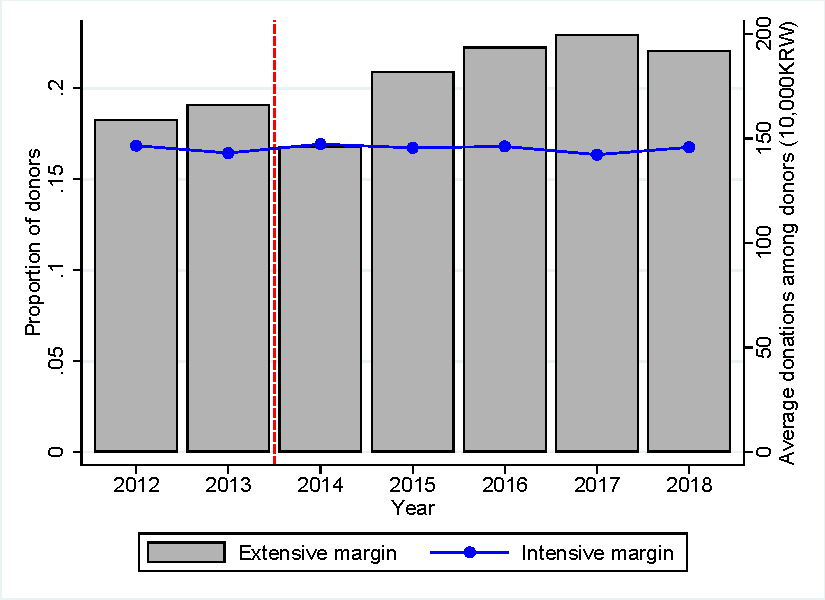
\includegraphics[width=0.9\linewidth]{C:/Users/katoo/Desktop/NASTAB/_assets/SummaryOutcome} 

  }

  \caption{Proportion of Donors and Average Donations among Donors}\label{fig:unnamed-chunk-1}
  \end{figure}

  \hypertarget{summary-statistics-of-covariates}{%
  \subsection{Summary Statistics of Covariates}\label{summary-statistics-of-covariates}}

  \begin{table}

  \caption{\label{tab:kableSummaryCovariate}Summary Statistics of Covariates}
  \centering
  \begin{tabular}[t]{lcccc}
  \toprule
   & 2012 & 2013 & 2014 & 2015\\
  \midrule
  Female & 0.51 & 0.51 & 0.52 & 0.52\\
  Age & 38.39 & 39.10 & 39.67 & 40.51\\
  Annual taxable income & 1699.86 & 1764.04 & 1838.76 & 1872.54\\
  University graduate & 0.28 & 0.28 & 0.29 & 0.30\\
  High school graduate & 0.30 & 0.30 & 0.31 & 0.31\\
  \#.Respondents & 14138 & 13984 & 13787 & 13524\\
  \#.Households & 4756 & 4807 & 4819 & 4832\\
  \bottomrule
  \end{tabular}
  \end{table}

  \hypertarget{summary-statistics-of-covariates-contd}{%
  \subsection{Summary Statistics of Covariates (Cont'd)}\label{summary-statistics-of-covariates-contd}}

  \begin{table}

  \caption{\label{tab:kableSummaryCovariate2}Summary Statistics of Covariates (Continued)}
  \centering
  \begin{tabular}[t]{lccc}
  \toprule
   & 2016 & 2017 & 2018\\
  \midrule
  Female & 0.52 & 0.52 & 0.52\\
  Age & 41.07 & 41.89 & 42.55\\
  Annual taxable income & 1906.91 & 1951.55 & 2039.47\\
  University graduate & 0.31 & 0.33 & 0.34\\
  High school graduate & 0.31 & 0.31 & 0.31\\
  \#.Respondents & 13238 & 12963 & 12795\\
  \#.Households & 4790 & 4770 & 4765\\
  \bottomrule
  \end{tabular}
  \end{table}

  \hypertarget{what-is-giving-price}{%
  \subsection{What is Giving Price?}\label{what-is-giving-price}}

  Consider allocation between private consumptions (\(x_i\)) and charitable giving (\(g_i\)).
  Let \(y_i\) be pre-tax total income.
  Then, the budget constraint is

  \[
      x_i + g_i = y_i - T_i(y_i, g_i),
  \]

  where \(T_i\) is tax amount depending on the pre-tax income and charitable giving.

  \hypertarget{determination-of-tax-amount}{%
  \subsection{Determination of Tax Amount}\label{determination-of-tax-amount}}

  Tax deduction reduces taxable income by giving, that is,

  \[
      T_i = \tau(y_i - g_i) \cdot (y_i - g_i),
  \]

  where \(\tau(\cdot)\) is the marginal income tax rate which is determined by \(y_i - g_i\).

  Tax credit reduces tax amount directly, that is,

  \[
      T_i = \tau(y_i)\cdot y_i - m g_i,
  \]

  where \(m \in [0, 1]\) is the tax credit rate.

  \hypertarget{derive-giving-price}{%
  \subsection{Derive Giving Price}\label{derive-giving-price}}

  Under the tax deduction system, the budget constraint is

  \[
      x_i + [1 - \tau(y_i - g_i)]g_i = [1 - \tau(y_i - g_i)] y_i.
  \]

  Thus, the giving price of tax deduction system is \(p_i^{d} = 1 - \tau(y_i - g_i)\).

  Under the tax credit system, the budget constraint is

  \[
      x_i + (1 - m) g_i = [1 - \tau(y_i)] y_i.
  \]

  Thus, the giving price of tax credit system is \(p_i^c = 1 - m\).

  \hypertarget{construct-giving-price}{%
  \subsection{Construct Giving Price}\label{construct-giving-price}}

  In the South Korea, the tax policy about charitable giving drastically changed in 2014.

  \begin{itemize}
  \tightlist
  \item
    tax deduction (before 2014): \(\text{Price}_i = 1 - \tau(y_i - g_i)\)

    \begin{itemize}
    \tightlist
    \item
      the giving price is endogenous because people can manipulate \(\tau(y_i - g_i)\) using the charitable giving \(g_i\). Since this problem is caused by \emph{last} donations, we use the giving price applying to the \emph{first} donations (\textbf{first price}). The first price is calculate by \(\tau(y_i)\) where \(y_i\) is the annual taxable income reported in the NaSTaB.
    \end{itemize}
  \item
    tax credit (after 2014): \(\text{Price}_i = 1 - m\)

    \begin{itemize}
    \tightlist
    \item
      In the South Korea, the tax credit rate determines exogeneity, \(m = 0.15\).
    \end{itemize}
  \end{itemize}

  \hypertarget{income-distribution-and-giving-price}{%
  \subsection{Income Distribution and Giving Price}\label{income-distribution-and-giving-price}}

  \begin{figure}

  {\centering 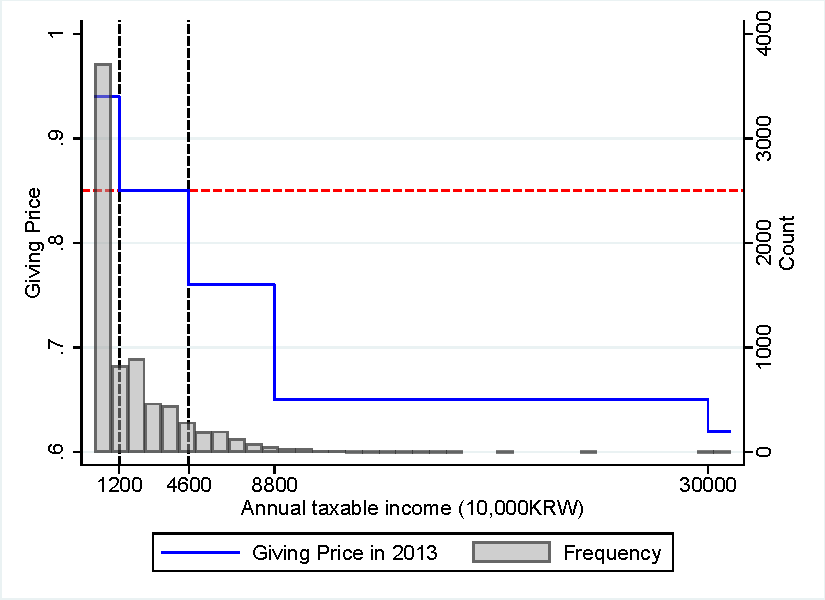
\includegraphics[width=0.9\linewidth]{C:/Users/katoo/Desktop/NASTAB/_assets/SummaryPriceChange} 

  }

  \caption{Income Distribution and Giving Price in 2013}\label{fig:unnamed-chunk-2}
  \end{figure}

  \hypertarget{time-series-of-average-donations-by-benefit-group}{%
  \subsection{Time Series of Average Donations By Benefit Group}\label{time-series-of-average-donations-by-benefit-group}}

  \begin{figure}

  {\centering 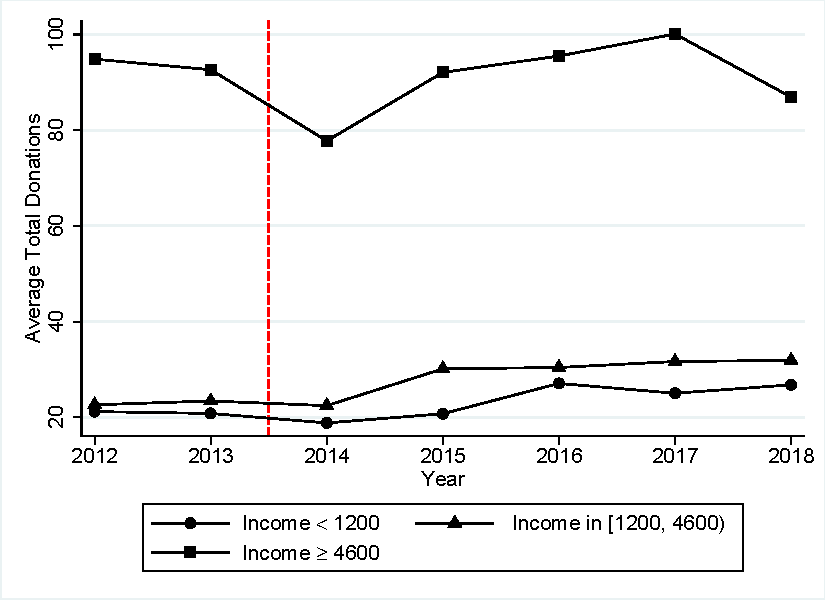
\includegraphics[width=0.9\linewidth]{C:/Users/katoo/Desktop/NASTAB/_assets/AverageDonationsByBenefitGroup} 

  }

  \caption{Time Series of Average Donations by Benefit Group}\label{fig:unnamed-chunk-3}
  \end{figure}

  \hypertarget{time-series-of-extensive-margin-by-benfit-group}{%
  \subsection{Time Series of Extensive Margin by Benfit Group}\label{time-series-of-extensive-margin-by-benfit-group}}

  \begin{figure}

  {\centering 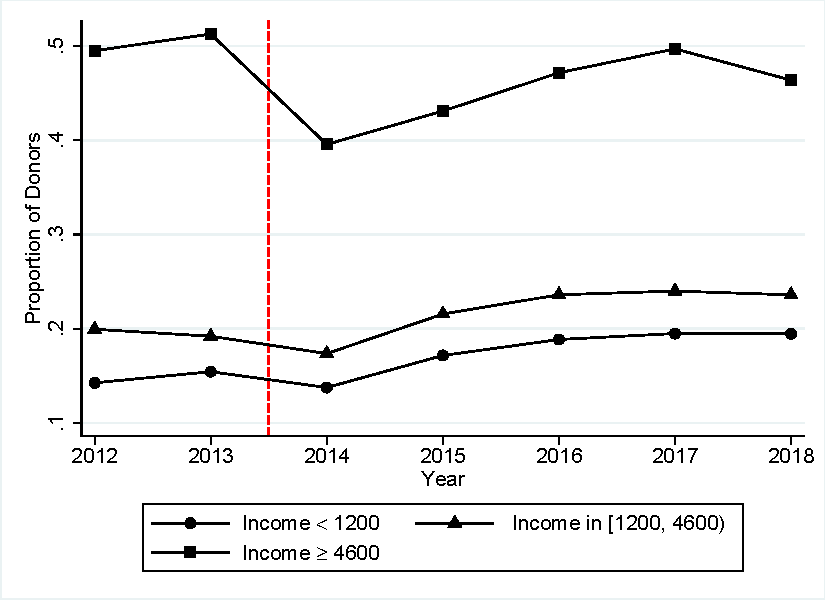
\includegraphics[width=0.9\linewidth]{C:/Users/katoo/Desktop/NASTAB/_assets/ExtensiveByBenefitGroup} 

  }

  \caption{Time Series of Proportion of Donors by Benefit Group}\label{fig:unnamed-chunk-4}
  \end{figure}

  \hypertarget{time-series-of-intensive-margin-by-benfit-group}{%
  \subsection{Time Series of Intensive Margin by Benfit Group}\label{time-series-of-intensive-margin-by-benfit-group}}

  \begin{figure}

  {\centering 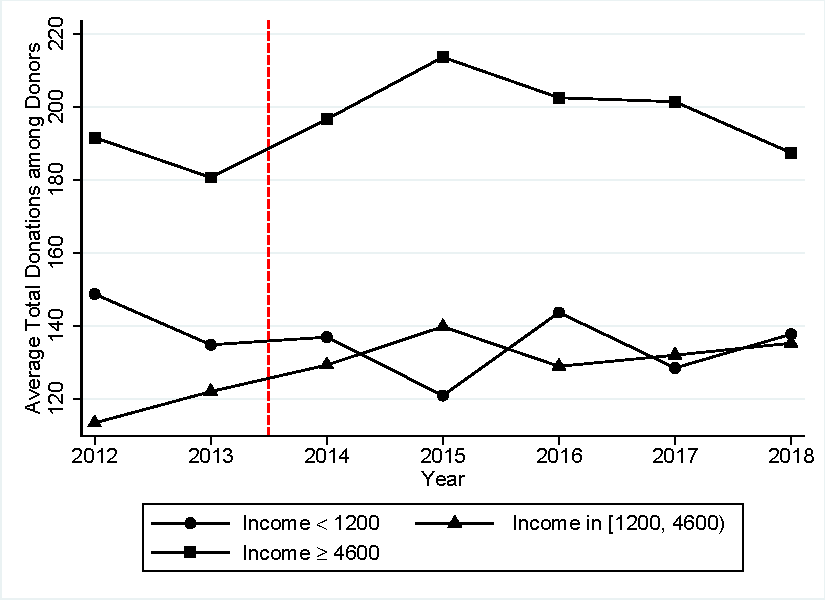
\includegraphics[width=0.9\linewidth]{C:/Users/katoo/Desktop/NASTAB/_assets/IntensiveByBenefitGroup} 

  }

  \caption{Time Series of Average Donations among Donors by Benefit Group}\label{fig:unnamed-chunk-5}
  \end{figure}

  \hypertarget{empirical-strategy}{%
  \subsection{Empirical Strategy}\label{empirical-strategy}}

  Our baseline regression equation is

  \[
      \log(\text{Giving}_{ijt}) = 
      \alpha_i + \beta_1 \log(\text{Price}_{ijt}) + \delta X_{ijt} + \lambda_t + \epsilon_{ijt}.
  \]

  \begin{itemize}
  \tightlist
  \item
    \(\log(\text{Giving}_{ijt})\) is logarithm of individual \(i\)'s charitable giving in year \(t\).
  \item
    \(\log(\text{Price}_{ijt})\) is logarithm of individual \(i\)'s giving price in year \(t\).
  \item
    \(\beta_1\) represents the price elasticity of giving.
  \item
    \(\alpha_i\) and \(\lambda_t\) are individual and time fixed effect, respectively.
  \end{itemize}

  \hypertarget{intensive-margin-and-extensive-margin}{%
  \subsection{Intensive Margin and Extensive Margin}\label{intensive-margin-and-extensive-margin}}

  Let \(D_{ijt}\) be a dummy variable taking 1 if individual \(i\) whose resident area \(j\) in year \(t\) donate in year \(t\)

  \begin{itemize}
  \tightlist
  \item
    Intensive margin: Estiamte \(\beta_1\) where outcome variable is \(\log(\text{Giving}_{ijt})\), using units with \(D_{ijt} = 1\).
  \item
    Extensive margin: Estimate \(\beta_1\) where outcome variable is \(D_{ijt}\).

    \begin{itemize}
    \tightlist
    \item
      Extensive-margin price elasticity can be calculated by \(\beta_1/\bar{D}\) where \(\bar{D}\) is the sample mean of \(D_{ijt}\).
    \end{itemize}
  \end{itemize}

  Covariates in each column corresponds to a column in a previous slide.

  \hypertarget{main-results}{%
  \section{Main Results}\label{main-results}}

  \hypertarget{price-and-income-elasticity}{%
  \subsection{Price and Income Elasticity}\label{price-and-income-elasticity}}

  \begin{table}

  \caption{\label{tab:kableEstimateElasticityPart1}Main Results}
  \centering
  \begin{threeparttable}
  \begin{tabular}[t]{lccccc}
  \toprule
   & (1) & (2) & (3) & (4) & (5)\\
  \midrule
  ln(giving price) & -1.071*** & -1.264*** & -1.298*** & -1.117*** & -1.121***\\
   & (0.201) & (0.212) & (0.229) & (0.228) & (0.228)\\
  Time FE & Y & Y & Y & Y & Y\\
  Age & N & Y & Y & Y & Y\\
  Year X Education & N & N & Y & Y & Y\\
  Year X Gender & N & N & N & Y & Y\\
  Resident Area & N & N & N & N & Y\\
  N & 54213 & 54213 & 54211 & 54211 & 54211\\
  \bottomrule
  \end{tabular}
  \begin{tablenotes}
  \item Notes: $^{*}$ $p < 0.1$, $^{**}$ $p < 0.05$, $^{***}$ $p < 0.01$. Standard errors are clustered at individual level. When controlling age, we alson include its squared term.
  \end{tablenotes}
  \end{threeparttable}
  \end{table}

  \begin{table}

  \caption{\label{tab:kableEstimateElasticityPart2}Main Results: Intensive- and Extensive-Margin Elasticity}
  \centering
  \begin{threeparttable}
  \begin{tabular}[t]{lccccc}
  \toprule
   & (1) & (2) & (3) & (4) & (5)\\
  \midrule
  \addlinespace[0.3em]
  \multicolumn{6}{l}{\textbf{Intensive-Margin Elasticity}}\\
  \hspace{1em}ln(giving price) & -0.593*** & -0.843*** & -1.022*** & -0.887*** & -0.891***\\
  \hspace{1em} & (0.202) & (0.212) & (0.231) & (0.242) & (0.243)\\
  \hspace{1em}N & 11704 & 11704 & 11704 & 11704 & 11704\\
  \addlinespace[0.3em]
  \multicolumn{6}{l}{\textbf{Extensive-Margin Elasticity}}\\
  \hspace{1em}ln(giving price) & -0.258*** & -0.290*** & -0.274*** & -0.238*** & -0.239***\\
  \hspace{1em} & (0.046) & (0.048) & (0.052) & (0.052) & (0.052)\\
  \hspace{1em}Price elasticity at mean & -1.699*** & -1.907*** & -1.807*** & -1.569*** & -1.573***\\
  \hspace{1em} & (0.301) & (0.316) & (0.341) & (0.341) & (0.341)\\
  \hspace{1em}Time FE & Y & Y & Y & Y & Y\\
  \hspace{1em}Age & N & Y & Y & Y & Y\\
  \hspace{1em}Year X Education & N & N & Y & Y & Y\\
  \hspace{1em}Year X Gender & N & N & N & Y & Y\\
  \hspace{1em}Resident Area & N & N & N & N & Y\\
  \hspace{1em}N & 54213 & 54213 & 54211 & 54211 & 54211\\
  \bottomrule
  \end{tabular}
  \begin{tablenotes}
  \item Notes: $^{*}$ $p < 0.1$, $^{**}$ $p < 0.05$, $^{***}$ $p < 0.01$. Standard errors are clustered at individual level. When controlling age, we alson include its squared term. The implied extensive-marign price elasticity is evaluated at the sample mean of $D_{ijt}$.
  \end{tablenotes}
  \end{threeparttable}
  \end{table}

  \hypertarget{robustness-check}{%
  \subsection{Robustness Check}\label{robustness-check}}

  \begin{table}

  \caption{\label{tab:kablePanelIVEstimateElasticity}Panel IV Results}
  \centering
  \begin{threeparttable}
  \begin{tabular}[t]{lccc}
  \toprule
  \multicolumn{1}{c}{Lag $k$} & \multicolumn{1}{c}{$k = 1$} & \multicolumn{1}{c}{$k = 2$} & \multicolumn{1}{c}{$k = 3$} \\
  \cmidrule(l{3pt}r{3pt}){1-1} \cmidrule(l{3pt}r{3pt}){2-2} \cmidrule(l{3pt}r{3pt}){3-3} \cmidrule(l{3pt}r{3pt}){4-4}
   & (1) & (2) & (3)\\
  \midrule
  ln(giving price) & -1.279*** & -1.155*** & -1.150***\\
   & (0.478) & (0.414) & (0.369)\\
  Individual FE & Y & Y & Y\\
  Time FE & Y & Y & Y\\
  Other Controls & Y & Y & Y\\
  F-stat of IV & 10315.94 & 11506.64 & 11569.61\\
  N & 51548 & 49217 & 46399\\
  \bottomrule
  \end{tabular}
  \begin{tablenotes}
  \item Notes: $^{*}$ $p < 0.1$, $^{**}$ $p < 0.05$, $^{***}$ $p < 0.01$. Standard errors are clustered at individual level. Other controls are age (its squared value), the interaction between year dummies and education dummies, the interaction between year dummies and gender dummies, and resident area. The instumental variable is $\log(\text{Price}_{ijt}/\text{Price}_{ij(t-k)})$.
  \end{tablenotes}
  \end{threeparttable}
  \end{table}

  \begin{table}

  \caption{\label{tab:kablePanelIVEstimateElasticityIntExt}Panel IV Results: Intensive- and Extensive-Margin Elasticity}
  \centering
  \begin{threeparttable}
  \begin{tabular}[t]{lccc}
  \toprule
  \multicolumn{1}{c}{Lag $k$} & \multicolumn{1}{c}{$k = 1$} & \multicolumn{1}{c}{$k = 2$} & \multicolumn{1}{c}{$k = 3$} \\
  \cmidrule(l{3pt}r{3pt}){1-1} \cmidrule(l{3pt}r{3pt}){2-2} \cmidrule(l{3pt}r{3pt}){3-3} \cmidrule(l{3pt}r{3pt}){4-4}
   & (1) & (2) & (3)\\
  \midrule
  \addlinespace[0.3em]
  \multicolumn{4}{l}{\textbf{Intensive Margin}}\\
  \hspace{1em}ln(giving price) & -0.0004 & 0.0261 & -0.4378\\
  \hspace{1em} & (0.5687) & (0.4410) & (0.3763)\\
  \hspace{1em}F-stat of IV & 1679.78 & 2040.66 & 2419.05\\
  \hspace{1em}N & 11332 & 10954 & 10451\\
  \addlinespace[0.3em]
  \multicolumn{4}{l}{\textbf{Extensive Margin}}\\
  \hspace{1em}ln(giving price) & -0.3036*** & -0.2944*** & -0.2472***\\
  \hspace{1em} & (0.1101) & (0.0934) & (0.0847)\\
  \hspace{1em}Price elasticity at mean & -2.000*** & -1.939*** & -1.628***\\
  \hspace{1em} & (0.725) & (0.615) & (0.558)\\
  \hspace{1em}Individual FE & Y & Y & Y\\
  \hspace{1em}Time FE & Y & Y & Y\\
  \hspace{1em}Other Controls & Y & Y & Y\\
  \hspace{1em}F-stat of IV & 10315.94 & 11506.64 & 11569.61\\
  \hspace{1em}N & 51548 & 49217 & 46399\\
  \bottomrule
  \end{tabular}
  \begin{tablenotes}
  \item Notes: $^{*}$ $p < 0.1$, $^{**}$ $p < 0.05$, $^{***}$ $p < 0.01$. Standard errors are clustered at individual level. Other controls are age (its squared value), the interaction between year dummies and education dummies, the interaction between year dummies and gender dummies, and resident area. The instumental variable is $\log(\text{Price}_{ijt}/\text{Price}_{ij(t-k)})$. The implied extensive-marign price elasticity is evaluated at the sample mean of $D_{ijt}$.
  \end{tablenotes}
  \end{threeparttable}
  \end{table}

  \begin{table}

  \caption{\label{tab:kableShortEstimateElasticity}Results with 2013 and 2014 Data}
  \centering
  \begin{threeparttable}
  \begin{tabular}[t]{lcccc}
  \toprule
  \multicolumn{1}{c}{Model} & \multicolumn{1}{c}{FE} & \multicolumn{3}{c}{Panel IV} \\
  \cmidrule(l{3pt}r{3pt}){1-1} \cmidrule(l{3pt}r{3pt}){2-2} \cmidrule(l{3pt}r{3pt}){3-5}
  \multicolumn{1}{c}{Lag $k$} & \multicolumn{1}{c}{ } & \multicolumn{1}{c}{$k = 1$} & \multicolumn{1}{c}{$k = 2$} & \multicolumn{1}{c}{$k = 3$} \\
  \cmidrule(l{3pt}r{3pt}){1-1} \cmidrule(l{3pt}r{3pt}){3-3} \cmidrule(l{3pt}r{3pt}){4-4} \cmidrule(l{3pt}r{3pt}){5-5}
   & (1) & (2) & (3) & (4)\\
  \midrule
  ln(giving price) & -1.466*** & -1.535*** & -1.683*** & -1.151***\\
   & (0.327) & (0.360) & (0.378) & (0.385)\\
  Individual FE & Y & Y & Y & Y\\
  Time FE & Y & Y & Y & Y\\
  Other Controls & Y & Y & Y & Y\\
  F-stat of IV &  & 7420.10 & 4490.74 & 5034.58\\
  N & 15134 & 13727 & 12902 & 12420\\
  \bottomrule
  \end{tabular}
  \begin{tablenotes}
  \item Notes: $^{*}$ $p < 0.1$, $^{**}$ $p < 0.05$, $^{***}$ $p < 0.01$. Standard errors are clustered at individual level. Other controls are age (its squared value), the interaction between year dummies and education dummies, the interaction between year dummies and gender dummies, and resident area. The instumental variable is $\log(\text{Price}_{ijt}/\text{Price}_{ij(t-k)})$.
  \end{tablenotes}
  \end{threeparttable}
  \end{table}

  \begin{table}

  \caption{\label{tab:kableShortEstimateElasticityIntExt}Intensive- and Extensive-Margin Elasticity with 2013 and 2014 Data}
  \centering
  \begin{threeparttable}
  \begin{tabular}[t]{lcccc}
  \toprule
  \multicolumn{1}{c}{Model} & \multicolumn{1}{c}{FE} & \multicolumn{3}{c}{Panel IV with FE} \\
  \cmidrule(l{3pt}r{3pt}){1-1} \cmidrule(l{3pt}r{3pt}){2-2} \cmidrule(l{3pt}r{3pt}){3-5}
  \multicolumn{1}{c}{Lag $k$} & \multicolumn{1}{c}{ } & \multicolumn{1}{c}{$k = 1$} & \multicolumn{1}{c}{$k = 2$} & \multicolumn{1}{c}{$k = 3$} \\
  \cmidrule(l{3pt}r{3pt}){1-1} \cmidrule(l{3pt}r{3pt}){3-3} \cmidrule(l{3pt}r{3pt}){4-4} \cmidrule(l{3pt}r{3pt}){5-5}
   & (1) & (2) & (3) & (4)\\
  \midrule
  \addlinespace[0.3em]
  \multicolumn{5}{l}{\textbf{Intensive Margin}}\\
  \hspace{1em}ln(giving price) & -0.759** & -0.736* & -0.819** & -0.543\\
  \hspace{1em} & (0.344) & (0.418) & (0.404) & (0.371)\\
  \hspace{1em}F-stat of IV &  & 1920.08 & 1762.03 & 1706.53\\
  \hspace{1em}N & 2938 & 2746 & 2615 & 2512\\
  \addlinespace[0.3em]
  \multicolumn{5}{l}{\textbf{Extensive Margin}}\\
  \hspace{1em}ln(giving price) & -0.332*** & -0.341*** & -0.380*** & -0.291***\\
  \hspace{1em} & (0.074) & (0.083) & (0.085) & (0.089)\\
  \hspace{1em}Elasticity & -2.186*** & -2.249*** & -2.504*** & -1.920***\\
  \hspace{1em} & (0.488) & (0.547) & (0.559) & (0.583)\\
  \hspace{1em}Individual FE & Y & Y & Y & Y\\
  \hspace{1em}Time FE & Y & Y & Y & Y\\
  \hspace{1em}Other Controls & Y & Y & Y & Y\\
  \hspace{1em}F-stat of IV &  & 7420.10 & 4490.74 & 5034.58\\
  \hspace{1em}N & 15134 & 13727 & 12902 & 12420\\
  \bottomrule
  \end{tabular}
  \begin{tablenotes}
  \item Notes: $^{*}$ $p < 0.1$, $^{**}$ $p < 0.05$, $^{***}$ $p < 0.01$. Standard errors are clustered at individual level. Other controls are age (its squared value), the interaction between year dummies and education dummies, the interaction between year dummies and gender dummies, and resident area. The instumental variable is $\log(\text{Price}_{ijt}/\text{Price}_{ij(t-k)})$. The implied extensive-marign price elasticity is evaluated at the sample mean of $D_{ijt}$.
  \end{tablenotes}
  \end{threeparttable}
  \end{table}

  \hypertarget{political-trust-and-price-elasticity}{%
  \section{Political Trust and Price Elasticity}\label{political-trust-and-price-elasticity}}

  \hypertarget{estimation-of-trust-index}{%
  \subsection{Estimation of Trust Index}\label{estimation-of-trust-index}}

  The trust for politicans is time-varying variable because it depends on governments' policies.
  We make time-invarying trust index using the fixed effect model.

  \[
      \text{Trust}_{ijt} = \text{Trustid}_{ij} + c_j \cdot \lambda_t + \lambda_t + \epsilon_{ijt}.
  \]

  \begin{itemize}
  \tightlist
  \item
    \(\text{Trust}_{ijt}\): trust for politicians (5-Likert scale)
  \item
    \(\text{Trustid}_i\): individual fixed effect (\textbf{Trust index})
  \item
    \(c_j \cdot \lambda_t\) captures local governments' policies effect
  \item
    \(\lambda_t\) captures the central government policies effect
  \end{itemize}

  \hypertarget{histrogram-of-trust-index}{%
  \subsection{Histrogram of Trust Index}\label{histrogram-of-trust-index}}

  \begin{figure}

  {\centering 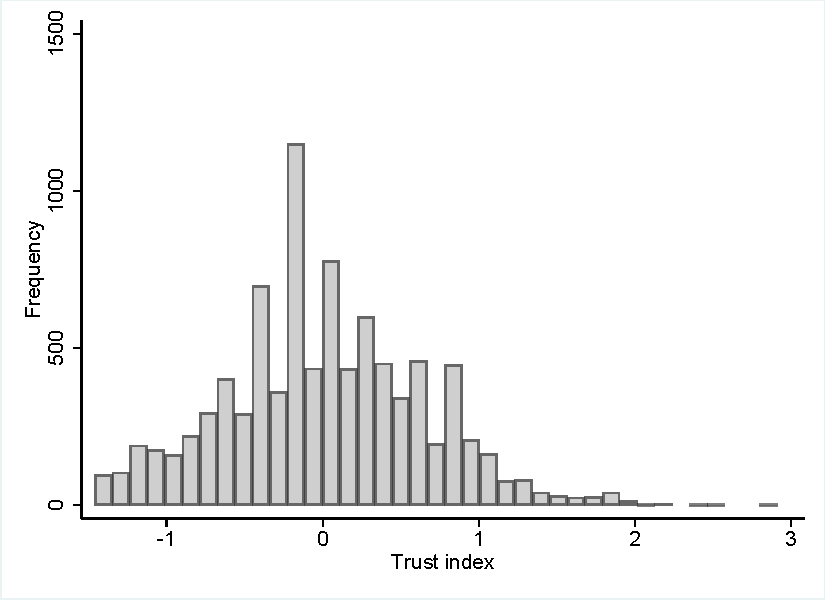
\includegraphics[width=0.9\linewidth]{C:/Users/katoo/Desktop/NASTAB/_assets/HistogramTrustid} 

  }

  \caption{Histogram of Trust Index}\label{fig:unnamed-chunk-6}
  \end{figure}

  \hypertarget{heterogenous-price-elasticity-by-political-trust}{%
  \subsection{Heterogenous Price Elasticity by Political Trust}\label{heterogenous-price-elasticity-by-political-trust}}

  To see the heterogenous price elasticity by political trust,
  We estimated the baseline regression model (5) (see Table \ref{tab:kableEstimateElasticity}),
  using sample grouped by the trust index.

  \begin{itemize}
  \tightlist
  \item
    Three quantile groups: we divide units \(i\) into the first, second, and third quantile of trust index (1Q, 2Q, and 3Q, respectively).
  \end{itemize}

  \hypertarget{trust-groups-descriptive-stats}{%
  \subsection{Trust Groups: Descriptive Stats}\label{trust-groups-descriptive-stats}}

  \begin{figure}

  {\centering 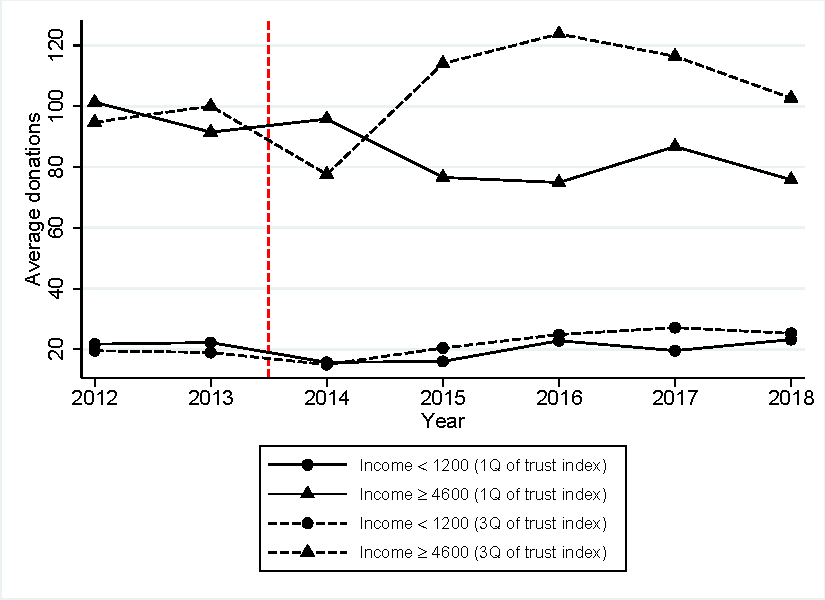
\includegraphics[width=0.9\linewidth]{C:/Users/katoo/Desktop/NASTAB/_assets/SummaryOutcomeByTrustGroup} 

  }

  \caption{Time Series of Average Donations by Subgroup}\label{fig:unnamed-chunk-7}
  \end{figure}

  \hypertarget{trust-groups-descriptive-statis-extensive-margin}{%
  \subsection{Trust Groups: Descriptive Statis (Extensive Margin)}\label{trust-groups-descriptive-statis-extensive-margin}}

  \begin{figure}

  {\centering 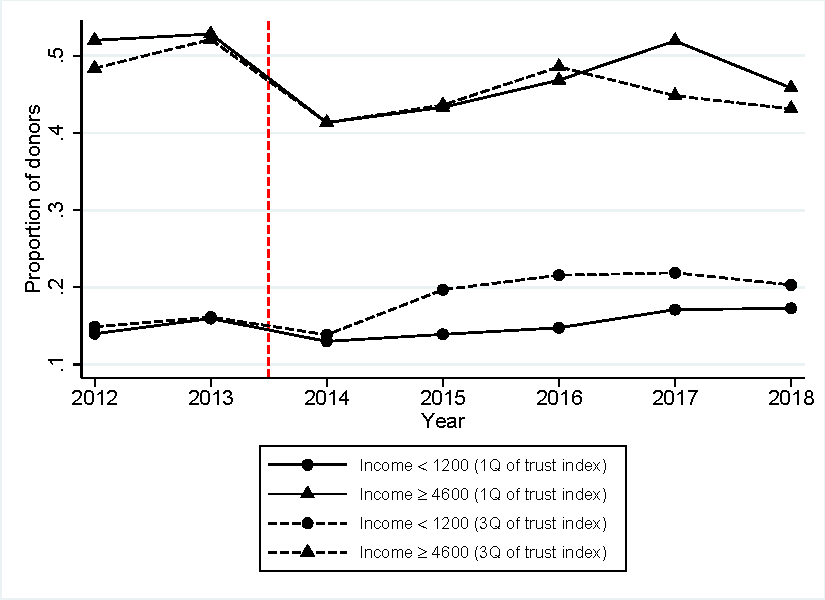
\includegraphics[width=0.9\linewidth]{C:/Users/katoo/Desktop/NASTAB/_assets/SummaryOutcomeExtensiveByTrustGroup} 

  }

  \caption{Time Series of Proportion of Donors by Subgroup}\label{fig:unnamed-chunk-8}
  \end{figure}

  \hypertarget{trust-groups-descriptive-stats-intensive-margin}{%
  \subsection{Trust Groups: Descriptive Stats (Intensive Margin)}\label{trust-groups-descriptive-stats-intensive-margin}}

  \begin{figure}

  {\centering 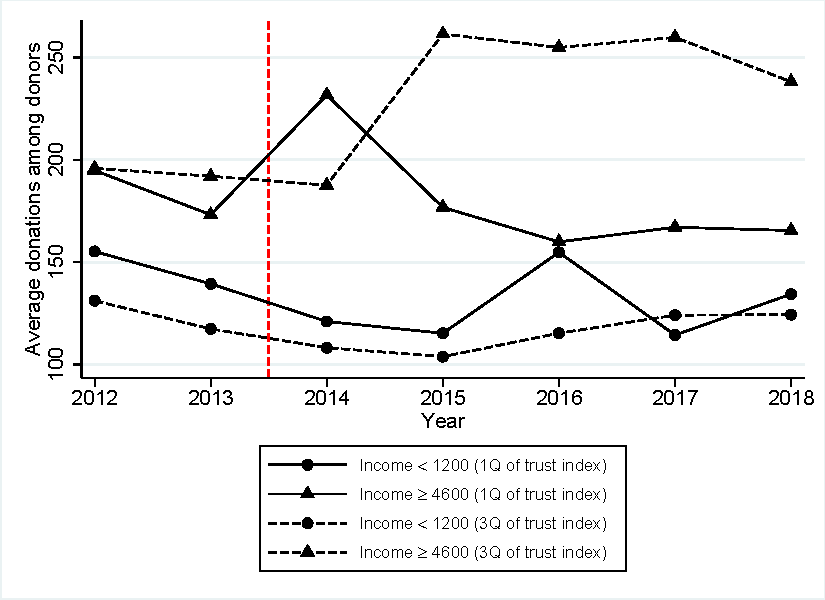
\includegraphics[width=0.9\linewidth]{C:/Users/katoo/Desktop/NASTAB/_assets/SummaryOutcomeIntensiveByTrustGroup} 

  }

  \caption{Time Series of Average Donations among Donors by Subgroup}\label{fig:unnamed-chunk-9}
  \end{figure}

  \hypertarget{trust-groups-estimation-result}{%
  \subsection{Trust Groups: Estimation Result}\label{trust-groups-estimation-result}}

  \begin{table}

  \caption{\label{tab:kableEstimateElasticityIntExtByTrustGroup3}Price Elasticity by Three Quantile Trust Groups}
  \centering
  \fontsize{8}{10}\selectfont
  \begin{tabular}[t]{lccc}
  \toprule
   & 1Q & 2Q & 3Q\\
  \midrule
  \addlinespace[0.3em]
  \multicolumn{4}{l}{\textbf{Overall}}\\
  \hspace{1em}ln(giving price) & -0.496 & -1.635*** & -1.157***\\
  \hspace{1em} & (0.398) & (0.391) & (0.410)\\
  \hspace{1em}N & 17421 & 16810 & \vphantom{1} 17075\\
  \addlinespace[0.3em]
  \multicolumn{4}{l}{\textbf{Intensive Margin}}\\
  \hspace{1em}ln(giving price) & -0.997** & -0.980** & -0.208\\
  \hspace{1em} & (0.408) & (0.398) & (0.450)\\
  \hspace{1em}N & 3516 & 3959 & 3917\\
  \addlinespace[0.3em]
  \multicolumn{4}{l}{\textbf{Extensive Margin}}\\
  \hspace{1em}ln(giving price) & -0.131 & -0.327*** & -0.244***\\
  \hspace{1em} & (0.089) & (0.090) & (0.093)\\
  \hspace{1em}Elasticity & -0.722 & -1.571*** & -1.088***\\
  \hspace{1em} & (0.487) & (0.433) & (0.416)\\
  \hspace{1em}N & 17421 & 16810 & 17075\\
  \bottomrule
  \end{tabular}
  \end{table}

  \hypertarget{robustness-check-1}{%
  \subsection{Robustness Check}\label{robustness-check-1}}

  \begin{enumerate}
  \def\labelenumi{\arabic{enumi}.}
  \tightlist
  \item
    Effect of presidential transition on trust index
  \item
    Effect of presidential transition on donation behavior
  \item
    Income and donations are determined simultaneously
  \item
    Last price elasticity
  \item
    Self-selection of receiving tax benefit
  \item
    Transitory and permanent elasticity
  \end{enumerate}

  \hypertarget{robustness-check-1-presidential-transition-effect-on-trust}{%
  \subsection{Robustness Check 1: Presidential Transition Effect on Trust}\label{robustness-check-1-presidential-transition-effect-on-trust}}

  \begin{itemize}
  \tightlist
  \item
    Even though we control time fixed effect when estimating the trust index, we may not rule out the effect of presidential transition on it perfectly.
  \item
    To check this point, we repeat estimate the same model using either data in 2015 and 2016 (Park's trust index) or in 2017 and 2018 (Moon's trust index), and obtain the president-specific trust indexs. After that, we test whether the average individual difference b/w these two indexs is statistically different from zero (pair-wise t-test).
  \item
    As a result, the average individual difference is -0.008 (s.e. = 0.01). This difference is not statistically different from zero (p-value = 0.446).
  \end{itemize}

  \hypertarget{robustness-check-2}{%
  \subsection{Robustness Check 2}\label{robustness-check-2}}

  We check the following two potential concerns

  \begin{itemize}
  \tightlist
  \item
    Presidential transition effect on donation behavior
  \item
    Income and donations are determined simultaneously
  \end{itemize}

  To address these problems, we estimate the FE model and Panel IV model with FE where instrument is \(\log(\text{Price}_{ijt}/\text{Price}_{ij(t-k)})\) for \(k = 1, 2, 3\), using data in 2013 and 2014.

  Note that f-statistics of IV is greater than 1000 when we estimate overall elasticity and extensive-margin elasticity, and greater than 400 when we estimate the intensive-margin elasticity.

  \hypertarget{robustness-check-2-result}{%
  \subsection{Robustness Check 2: Result}\label{robustness-check-2-result}}

  \begin{table}

  \caption{\label{tab:tabShortEstimateElasticityByTrustGroup3}Robustness Check of Heterogenous Price Elasiticity by Political Trust}
  \centering
  \fontsize{8}{10}\selectfont
  \begin{tabular}[t]{lccc}
  \toprule
   & 1Q & 2Q & 3Q\\
  \midrule
  \addlinespace[0.3em]
  \multicolumn{4}{l}{\textbf{FE Model}}\\
  \hspace{1em}ln(giving price) & -0.485 & -2.901*** & -1.164*\\
  \hspace{1em} & (0.564) & (0.563) & (0.623)\\
  \hspace{1em}N & 4713 & 4489 & 4586\\
  \addlinespace[0.3em]
  \multicolumn{4}{l}{\textbf{Panel IV (k = 1)}}\\
  \hspace{1em}ln(giving price) & -0.347 & -3.307*** & -1.242*\\
  \hspace{1em} & (0.639) & (0.602) & (0.656)\\
  \hspace{1em}N & 4337 & 4109 & 4190\\
  \addlinespace[0.3em]
  \multicolumn{4}{l}{\textbf{Panel IV (k = 2)}}\\
  \hspace{1em}ln(giving price) & -0.617 & -3.314*** & -1.204*\\
  \hspace{1em} & (0.627) & (0.689) & (0.702)\\
  \hspace{1em}N & 4100 & 3839 & 3975\\
  \addlinespace[0.3em]
  \multicolumn{4}{l}{\textbf{Panel IV (k = 3)}}\\
  \hspace{1em}ln(giving price) & -0.230 & -2.536*** & -0.807\\
  \hspace{1em} & (0.684) & (0.673) & (0.691)\\
  \hspace{1em}N & 3947 & 3700 & 3832\\
  \bottomrule
  \end{tabular}
  \end{table}

  \hypertarget{robustness-check-2-result-extensive-margin}{%
  \subsection{Robustness Check 2: Result (Extensive Margin)}\label{robustness-check-2-result-extensive-margin}}

  \begin{table}

  \caption{\label{tab:tabShortEstimateElasticityExtensiveByTrustGroup3}Robustness Check of Heterogenous Extensive-Margin Price Elasiticity by Political Trust}
  \centering
  \fontsize{8}{10}\selectfont
  \begin{tabular}[t]{lccc}
  \toprule
   & 1Q & 2Q & 3Q\\
  \midrule
  \addlinespace[0.3em]
  \multicolumn{4}{l}{\textbf{FE Model}}\\
  \hspace{1em}Implied Elasticity & -0.834 & -3.347*** & -1.386*\\
  \hspace{1em} & (0.728) & (0.672) & (0.774)\\
  \hspace{1em}N & 4713 & 4489 & 4586\\
  \addlinespace[0.3em]
  \multicolumn{4}{l}{\textbf{Panel IV (k = 1)}}\\
  \hspace{1em}Implied Elasticity & -0.438 & -3.880*** & -1.658*\\
  \hspace{1em} & (0.816) & (0.732) & (0.846)\\
  \hspace{1em}N & 4337 & 4109 & 4190\\
  \addlinespace[0.3em]
  \multicolumn{4}{l}{\textbf{Panel IV (k = 2)}}\\
  \hspace{1em}Implied Elasticity & -1.082 & -3.864*** & -1.223\\
  \hspace{1em} & (0.805) & (0.797) & (0.878)\\
  \hspace{1em}N & 4100 & 3839 & 3975\\
  \addlinespace[0.3em]
  \multicolumn{4}{l}{\textbf{Panel IV (k = 3)}}\\
  \hspace{1em}Implied Elasticity & -0.852 & -3.176*** & -0.850\\
  \hspace{1em} & (0.881) & (0.806) & (0.893)\\
  \hspace{1em}N & 3947 & 3700 & 3832\\
  \bottomrule
  \end{tabular}
  \end{table}

  \hypertarget{robustness-check-2-result-intensive-margin}{%
  \subsection{Robustness Check 2: Result (Intensive Margin)}\label{robustness-check-2-result-intensive-margin}}

  \begin{table}

  \caption{\label{tab:tabShortEstimateElasticityIntensiveByTrustGroup3}Robustness Check of Heterogenous Intenstive-Margin Price Elasiticity by Political Trust}
  \centering
  \fontsize{8}{10}\selectfont
  \begin{tabular}[t]{lccc}
  \toprule
   & 1Q & 2Q & 3Q\\
  \midrule
  \addlinespace[0.3em]
  \multicolumn{4}{l}{\textbf{FE Model}}\\
  \hspace{1em}ln(giving price) & -0.946* & -0.969* & -0.622\\
  \hspace{1em} & (0.540) & (0.575) & (0.673)\\
  \hspace{1em}N & 904 & 958 & 931\\
  \addlinespace[0.3em]
  \multicolumn{4}{l}{\textbf{Panel IV (k = 1)}}\\
  \hspace{1em}ln(giving price) & -1.408** & -0.687 & -0.396\\
  \hspace{1em} & (0.636) & (0.710) & (0.841)\\
  \hspace{1em}N & 847 & 898 & 881\\
  \addlinespace[0.3em]
  \multicolumn{4}{l}{\textbf{Panel IV (k = 2)}}\\
  \hspace{1em}ln(giving price) & -1.117* & -0.912 & -0.696\\
  \hspace{1em} & (0.651) & (0.657) & (0.787)\\
  \hspace{1em}N & 812 & 850 & 844\\
  \addlinespace[0.3em]
  \multicolumn{4}{l}{\textbf{Panel IV (k = 3)}}\\
  \hspace{1em}ln(giving price) & -0.640 & -0.611 & -0.327\\
  \hspace{1em} & (0.609) & (0.596) & (0.698)\\
  \hspace{1em}N & 777 & 819 & 816\\
  \bottomrule
  \end{tabular}
  \end{table}

  \hypertarget{governement-efficient-and-price-elasticity}{%
  \section{Governement Efficient and Price Elasticity}\label{governement-efficient-and-price-elasticity}}

  \hypertarget{government-efficiency}{%
  \subsection{Government Efficiency}\label{government-efficiency}}

  From the 2015 survey,
  NaSTaB asks the current and ideal balance between tax burden and welfare size.

  These variables provide us to investigate the relationship between price elasticity and govenrment's efficiency
  more directly.

  Thus, we did same excercise, using the current balance bewteen tax burden and welfare size.

  \hypertarget{construct-efficient-index}{%
  \subsection{Construct Efficient Index}\label{construct-efficient-index}}

  Questionnaire of tax-welfare balance index is

  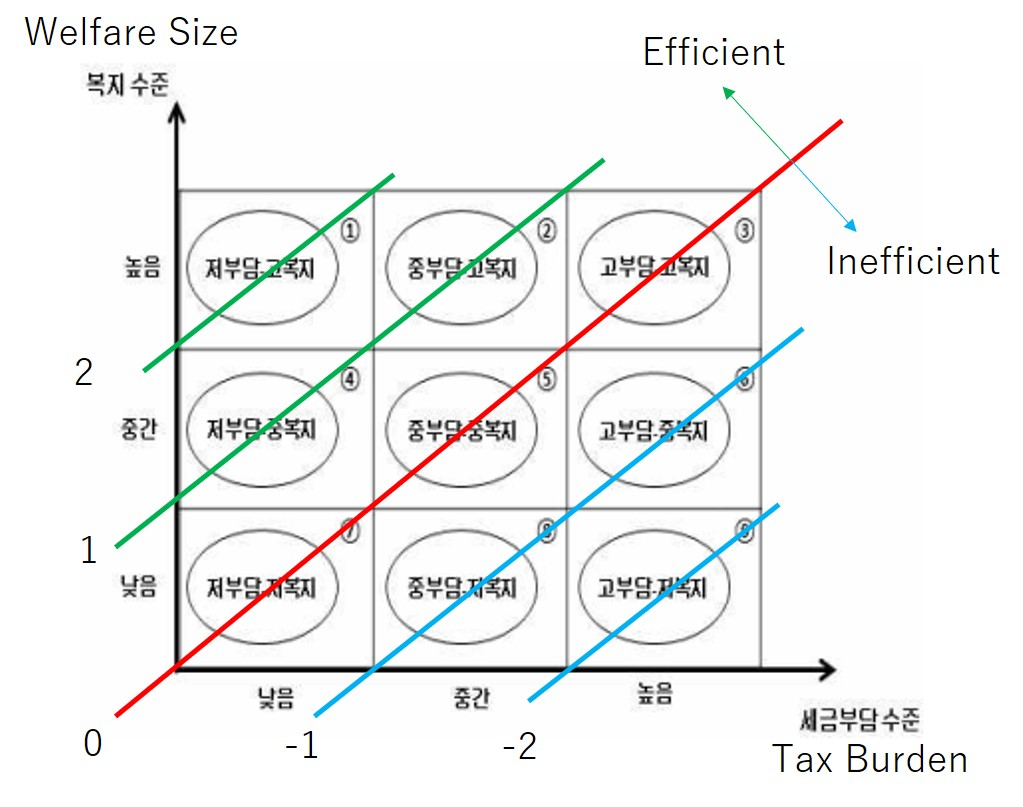
\includegraphics[width=0.5\textwidth,height=\textheight]{_assets/BalanceQuestion.jpg}

  To rule out government's policies, we use individual fixed effect as the \textbf{efficient index}

  \hypertarget{histrogram-of-efficient-index}{%
  \subsection{Histrogram of Efficient Index}\label{histrogram-of-efficient-index}}

  \begin{figure}

  {\centering 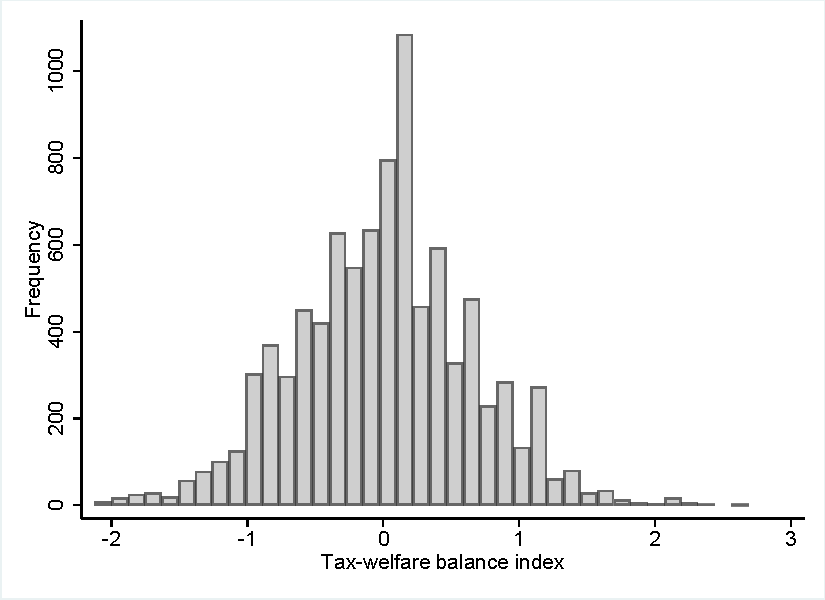
\includegraphics[width=0.9\linewidth]{C:/Users/katoo/Desktop/NASTAB/_assets/HistogramBalanceid} 

  }

  \caption{Histogram of Efficient Index}\label{fig:unnamed-chunk-10}
  \end{figure}

  \hypertarget{heterogenous-price-elasticity-by-governement-efficiency}{%
  \subsection{Heterogenous Price Elasticity by Governement Efficiency}\label{heterogenous-price-elasticity-by-governement-efficiency}}

  To see the heterogenous price elasticity by efficient index,
  We estimated the baseline regression model (5) (see Table \ref{tab:kableEstimateElasticity}),
  using sample grouped by the efficient index.

  \begin{itemize}
  \tightlist
  \item
    Three quantile groups: we divide units \(i\) into the first, second, and third quantile of efficient index (1Q, 2Q, and 3Q, respectively).
  \end{itemize}

  \hypertarget{efficient-groups-descriptive-stats}{%
  \subsection{Efficient Groups: Descriptive Stats}\label{efficient-groups-descriptive-stats}}

  \begin{figure}

  {\centering 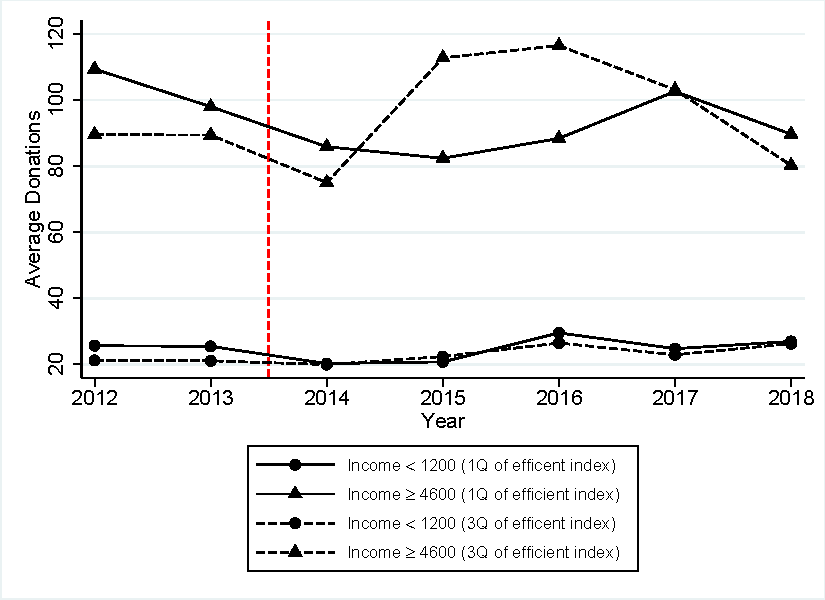
\includegraphics[width=0.9\linewidth]{C:/Users/katoo/Desktop/NASTAB/_assets/SummaryOutcomeByEfficientGroup3} 

  }

  \caption{Time Series of Average Donations by Subgroup}\label{fig:unnamed-chunk-11}
  \end{figure}

  \hypertarget{efficient-groups-descriptive-statis-extensive-margin}{%
  \subsection{Efficient Groups: Descriptive Statis (Extensive Margin)}\label{efficient-groups-descriptive-statis-extensive-margin}}

  \begin{figure}

  {\centering 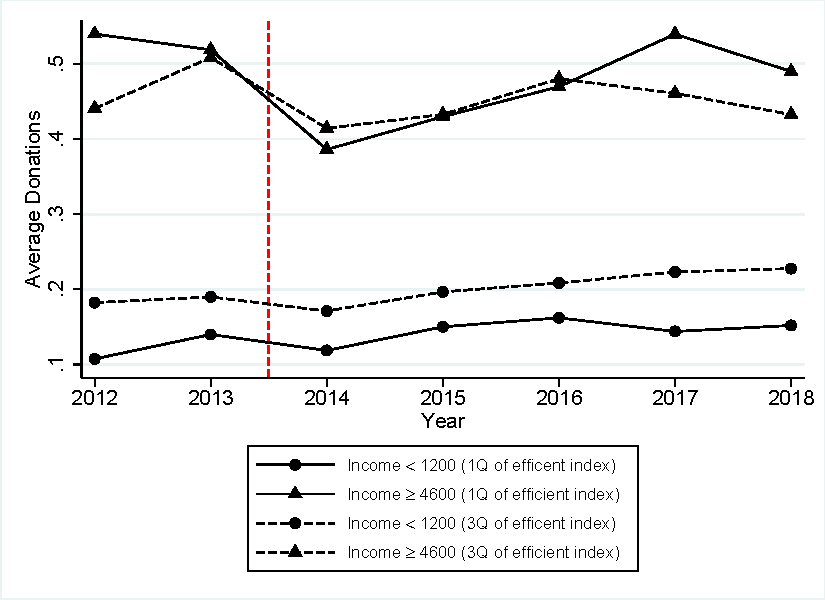
\includegraphics[width=0.9\linewidth]{C:/Users/katoo/Desktop/NASTAB/_assets/SummaryOutcomeExtensiveByEfficientGroup3} 

  }

  \caption{Time Series of Proportion of Donors by Subgroup}\label{fig:unnamed-chunk-12}
  \end{figure}

  \hypertarget{efficient-groups-descriptive-stats-intensive-margin}{%
  \subsection{Efficient Groups: Descriptive Stats (Intensive Margin)}\label{efficient-groups-descriptive-stats-intensive-margin}}

  \begin{figure}

  {\centering 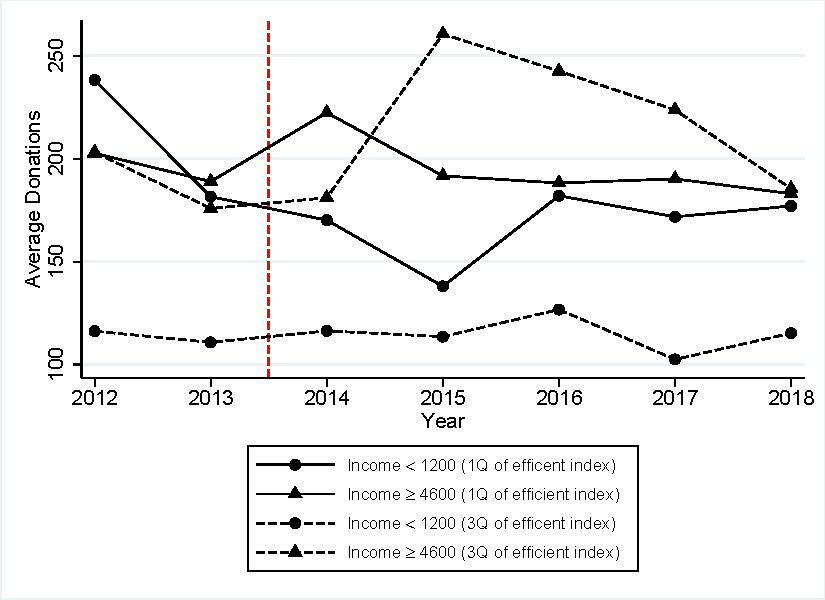
\includegraphics[width=0.9\linewidth]{C:/Users/katoo/Desktop/NASTAB/_assets/SummaryOutcomeIntensiveByEfficientGroup3} 

  }

  \caption{Time Series of Average Donations among Donors by Subgroup}\label{fig:unnamed-chunk-13}
  \end{figure}

  \hypertarget{efficient-groups-estimation-results}{%
  \subsection{Efficient Groups: Estimation Results}\label{efficient-groups-estimation-results}}

  \begin{table}

  \caption{\label{tab:kableEstimateElasticityByEfficientGroup3}Price Elasticity by Three Quantile Efficient Groups}
  \centering
  \fontsize{8}{10}\selectfont
  \begin{tabular}[t]{lccc}
  \toprule
   & 1Q & 2Q & 3Q\\
  \midrule
  \addlinespace[0.3em]
  \multicolumn{4}{l}{\textbf{Overall}}\\
  \hspace{1em}ln(giving price) & -1.321*** & -0.844** & -0.929**\\
  \hspace{1em} & (0.388) & (0.404) & (0.404)\\
  \hspace{1em}N & 17119 & 16662 & \vphantom{1} 17525\\
  \addlinespace[0.3em]
  \multicolumn{4}{l}{\textbf{Intensive Margin}}\\
  \hspace{1em}ln(giving price) & -0.792** & -0.360 & -1.111**\\
  \hspace{1em} & (0.383) & (0.423) & (0.497)\\
  \hspace{1em}N & 3696 & 3591 & 4105\\
  \addlinespace[0.3em]
  \multicolumn{4}{l}{\textbf{Extensive Margin}}\\
  \hspace{1em}ln(giving price) & -0.276*** & -0.225** & -0.174*\\
  \hspace{1em} & (0.087) & (0.094) & (0.091)\\
  \hspace{1em}Elasticity & -1.380*** & -1.115** & -0.787*\\
  \hspace{1em} & (0.435) & (0.466) & (0.412)\\
  \hspace{1em}N & 17119 & 16662 & 17525\\
  \bottomrule
  \end{tabular}
  \end{table}

  \hypertarget{robustness-check-3}{%
  \subsection{Robustness Check}\label{robustness-check-3}}

  \begin{enumerate}
  \def\labelenumi{\arabic{enumi}.}
  \tightlist
  \item
    Efficient index captures both government efficiency on concerns about budget deficits
  \item
    Effect of presidential transition on efficient index
  \item
    Effect of presidential transition on donation behavior
  \item
    Income and donations are determined simultaneously
  \item
    Last price elasticity
  \item
    Self-selection of receiving tax benefit
  \item
    Transitory and permanent elasticity
  \end{enumerate}

  \hypertarget{robustness-check-1-1}{%
  \subsection{Robustness Check 1}\label{robustness-check-1-1}}

  \begin{itemize}
  \tightlist
  \item
    Efficient index may capture both government efficiency on concerns about budget deficits

    \begin{itemize}
    \tightlist
    \item
      NASTAB asks respondents to answer the ideal balance b/w tax burdern and welfare size.
    \item
      We constructed the \textbf{ideal} efficient index, using the FE model to estimate the efficient index.
    \item
      We droped units with the ideal efficient index is less than 0 from each quantile group and repeated the same excercise.
    \item
      This is because respondents whose the ideal efficient index is less than 0 think governments should try to avoid budget deficits (high tax, low welfare).
    \end{itemize}
  \item
    Presidential transition effect on perceived efficiency

    \begin{itemize}
    \tightlist
    \item
      We constructed president-specific (ideal) efficient index and implemented the pair-wise t-test.
    \item
      As a result, average difference of these two indexs are not statistically siginificant zero.
    \end{itemize}
  \end{itemize}

  \hypertarget{robustness-check-1-estimation-results}{%
  \subsection{Robustness Check 1: Estimation Results}\label{robustness-check-1-estimation-results}}

  \begin{table}

  \caption{\label{tab:kableEstimateElasticityByPositiveEfficientGroup3}Heterogenous Price Elasticity by Efficiency Using Units with Ideal Efficient Index > 0}
  \centering
  \fontsize{8}{10}\selectfont
  \begin{tabular}[t]{lccc}
  \toprule
   & 1Q & 2Q & 3Q\\
  \midrule
  \addlinespace[0.3em]
  \multicolumn{4}{l}{\textbf{Overall}}\\
  \hspace{1em}ln(giving price) & -1.996*** & -1.122* & -0.063\\
  \hspace{1em} & (0.648) & (0.597) & (0.488)\\
  \hspace{1em}N & 7527 & 6900 & \vphantom{1} 9339\\
  \addlinespace[0.3em]
  \multicolumn{4}{l}{\textbf{Intensive Margin}}\\
  \hspace{1em}ln(giving price) & -1.138* & -0.900 & -0.952\\
  \hspace{1em} & (0.640) & (0.652) & (0.741)\\
  \hspace{1em}N & 1541 & 1474 & 2023\\
  \addlinespace[0.3em]
  \multicolumn{4}{l}{\textbf{Extensive Margin}}\\
  \hspace{1em}ln(giving price) & -0.317** & -0.220 & 0.014\\
  \hspace{1em} & (0.136) & (0.137) & (0.119)\\
  \hspace{1em}Elasticity & -1.582** & -1.091 & 0.062\\
  \hspace{1em} & (0.681) & (0.679) & (0.537)\\
  \hspace{1em}N & 7527 & 6900 & 9339\\
  \bottomrule
  \end{tabular}
  \end{table}

  \hypertarget{robustness-check-2-1}{%
  \subsection{Robustness Check 2}\label{robustness-check-2-1}}

  We check the following two potential concerns

  \begin{itemize}
  \tightlist
  \item
    Presidential transition effect on donation behavior
  \item
    Income and donations are determined simultaneously
  \end{itemize}

  To address these problems, we estimated the FE model and Panel IV model with FE where instrument is \(\log(\text{Price}_{ijt}/\text{Price}_{ij(t-k)})\) for \(k = 1, 2, 3\), using data in 2013 and 2014.
  Moreover, we droped units with the ideal efficient index \textless{} 0 from each quantile group.

  Note that f-statistics of IV is greater than 500 when we estimate overall elasticity and extensive-margin elasticity, and greater than 100 when we estimate the intensive-margin elasticity.

  \hypertarget{robustness-check-2-result-1}{%
  \subsection{Robustness Check 2: Result}\label{robustness-check-2-result-1}}

  \begin{table}

  \caption{\label{tab:tabShortEstimateElasticityByEfficientGroup3}Robustness Check of Heterogenous Price Elasiticity by Government Efficiency}
  \centering
  \fontsize{8}{10}\selectfont
  \begin{tabular}[t]{lccc}
  \toprule
   & 1Q & 2Q & 3Q\\
  \midrule
  \addlinespace[0.3em]
  \multicolumn{4}{l}{\textbf{FE Model}}\\
  \hspace{1em}ln(giving price) & -1.989** & -1.047 & -1.881**\\
  \hspace{1em} & (0.913) & (1.078) & (0.835)\\
  \hspace{1em}N & 2021 & 1841 & 2504\\
  \addlinespace[0.3em]
  \multicolumn{4}{l}{\textbf{Panel IV (k = 1)}}\\
  \hspace{1em}ln(giving price) & -1.881* & -1.093 & -2.189**\\
  \hspace{1em} & (0.992) & (1.272) & (0.851)\\
  \hspace{1em}N & 1842 & 1689 & 2292\\
  \addlinespace[0.3em]
  \multicolumn{4}{l}{\textbf{Panel IV (k = 2)}}\\
  \hspace{1em}ln(giving price) & -1.958* & -1.594 & -1.684\\
  \hspace{1em} & (1.101) & (1.212) & (1.024)\\
  \hspace{1em}N & 1723 & 1582 & 2174\\
  \addlinespace[0.3em]
  \multicolumn{4}{l}{\textbf{Panel IV (k = 3)}}\\
  \hspace{1em}ln(giving price) & -1.608 & -0.317 & -1.544\\
  \hspace{1em} & (1.079) & (1.219) & (0.999)\\
  \hspace{1em}N & 1645 & 1529 & 2096\\
  \bottomrule
  \end{tabular}
  \end{table}

  \hypertarget{robustness-check-2-result-extensive-margin-1}{%
  \subsection{Robustness Check 2: Result (Extensive Margin)}\label{robustness-check-2-result-extensive-margin-1}}

  \begin{table}

  \caption{\label{tab:tabShortEstimateElasticityExtensiveByEfficientGroup3}Robustness Check of Heterogenous Extensive-Margin Price Elasiticity by Government Efficiency}
  \centering
  \fontsize{8}{10}\selectfont
  \begin{tabular}[t]{lccc}
  \toprule
   & 1Q & 2Q & 3Q\\
  \midrule
  \addlinespace[0.3em]
  \multicolumn{4}{l}{\textbf{FE Model}}\\
  \hspace{1em}Implied Elasticity & -1.558 & -0.649 & -2.453**\\
  \hspace{1em} & (1.119) & (1.326) & (1.147)\\
  \hspace{1em}N & 2021 & 1841 & 2504\\
  \addlinespace[0.3em]
  \multicolumn{4}{l}{\textbf{Panel IV (k = 1)}}\\
  \hspace{1em}Implied Elasticity & -1.345 & -0.517 & -2.934**\\
  \hspace{1em} & (1.255) & (1.612) & (1.180)\\
  \hspace{1em}N & 1842 & 1689 & 2292\\
  \addlinespace[0.3em]
  \multicolumn{4}{l}{\textbf{Panel IV (k = 2)}}\\
  \hspace{1em}Implied Elasticity & -1.396 & -1.557 & -1.998\\
  \hspace{1em} & (1.264) & (1.486) & (1.439)\\
  \hspace{1em}N & 1723 & 1582 & 2174\\
  \addlinespace[0.3em]
  \multicolumn{4}{l}{\textbf{Panel IV (k = 3)}}\\
  \hspace{1em}Implied Elasticity & -1.056 & -0.460 & -1.795\\
  \hspace{1em} & (1.262) & (1.477) & (1.355)\\
  \hspace{1em}N & 1645 & 1529 & 2096\\
  \bottomrule
  \end{tabular}
  \end{table}

  \hypertarget{robustness-check-2-result-intensive-margin-1}{%
  \subsection{Robustness Check 2: Result (Intensive Margin)}\label{robustness-check-2-result-intensive-margin-1}}

  \begin{table}

  \caption{\label{tab:tabShortEstimateElasticityIntensiveByEfficientGroup3}Robustness Check of Heterogenous Intenstive-Margin Price Elasiticity by Government Efficiency}
  \centering
  \fontsize{8}{10}\selectfont
  \begin{tabular}[t]{lccc}
  \toprule
   & 1Q & 2Q & 3Q\\
  \midrule
  \addlinespace[0.3em]
  \multicolumn{4}{l}{\textbf{FE Model}}\\
  \hspace{1em}ln(giving price) & -0.753 & -2.301* & -1.362\\
  \hspace{1em} & (0.848) & (1.310) & (0.956)\\
  \hspace{1em}N & 404 & 361 & 479\\
  \addlinespace[0.3em]
  \multicolumn{4}{l}{\textbf{Panel IV (k = 1)}}\\
  \hspace{1em}ln(giving price) & -0.749 & -3.220* & -1.471\\
  \hspace{1em} & (1.088) & (1.812) & (1.013)\\
  \hspace{1em}N & 380 & 340 & 449\\
  \addlinespace[0.3em]
  \multicolumn{4}{l}{\textbf{Panel IV (k = 2)}}\\
  \hspace{1em}ln(giving price) & -0.770 & -1.216 & -0.771\\
  \hspace{1em} & (0.997) & (1.504) & (0.966)\\
  \hspace{1em}N & 357 & 322 & 433\\
  \addlinespace[0.3em]
  \multicolumn{4}{l}{\textbf{Panel IV (k = 3)}}\\
  \hspace{1em}ln(giving price) & 0.573 & -0.691 & -1.472\\
  \hspace{1em} & (1.117) & (1.088) & (0.991)\\
  \hspace{1em}N & 337 & 307 & 414\\
  \bottomrule
  \end{tabular}
  \end{table}

  \hypertarget{conclusions}{%
  \section{Conclusions}\label{conclusions}}

  \hypertarget{conclusions-1}{%
  \subsection{Conclusions}\label{conclusions-1}}

  \clearpage

  \hypertarget{references}{%
  \subsection*{References}\label{references}}
  \addcontentsline{toc}{subsection}{References}

\end{document}

